\chapter{Special Probability Distributions}

\section{Discrete Uniform Distribution}

\begin{definition}[Discrete Uniform Distribution]
If the random variable $X$ assumes the values $x_1, x_2, \dots x_k$ with equal probability, then the random variable $X$ is said to have a discrete uniform distribution and the probability function is given by 
$$
f_X(x) = 
\begin{cases}
\dfrac{1}{k}, \text{ if } x = x_1, x_2, \dots x_k \\
0, \qquad \text{ otherwise}
\end{cases}
$$
\end{definition}
\thm{Mean and Variance of Discrete Uniform Distribution \\
\begin{equation*}
\begin{split}
    \mu &= E(X) = \sum_{all\ x} x f_X(x) = \sum_{i = 1}^k x_i \dfrac{1}{k} = \dfrac{1}{k} \sum_{i = 1}^k x_i \\
    \sigma^2 &= V(X) = \sum_{all \ x} (x-\mu)^2 f_X(x) = \dfrac{1}{k}\sum_{i = 1}^k (x_i - \mu)^2 \\
    \text{Alternatively,} \\
    \sigma^2 &= E(X^2) - \mu^2 = \dfrac{1}{k}\left( \sum_{i = 1}^k x_i^2 \right) - \mu^2
\end{split}
\end{equation*}
}
\section{Bernoulli and Binomial Distribution}

\begin{definition}[Bernoulli Experiment]
A Bernoulli experiment is a random experiment with only 2 possible outcomes, say "success" or "failure" (e.g. head or tail, defective or non-defective, boy or girl, yes or no). It is convenient to code the 2 outcomes as 1 and 0.
\end{definition}

\begin{definition}[Bernoulli Distribution]
A random variable $X$ is defined to have a Bernoulli distribution if the probability function of $X$ is given by 
$$
f_X(x) = \begin{cases}
p^x(1-p)^{1-x}, \  x = 0,1 \\
0, \qquad \text{ otherwise}
\end{cases}
$$ where the parameter $p$ satisfies the $0 < p < 1$
\end{definition}

\begin{note}
\end{note}
\begin{itemize}
    \item $(1-p)$ is often denoted by $q$.
    \item $P(X = 1) = p$ and $P(X = 0) = 1 - p = q$
    \item We code any outcome that we consider to be a success to be 1, and all other outcomes (that we consider to be failures) to be 0. This is why the only possible values of $x$ are 0 and 1. For example, if we are interested in finding the number of red balls being drawn from a box then we will code any selection that results in a red ball being drawn to be 1, and all non-red balls to be 0.
\end{itemize}

\begin{note}[Parameter and Family of Distributions]
\end{note}
Suppose $f_X(x)$ depends on a quantity that can be assigned any one of a number of possible values, with each different value determining a different probability distribution. Such a quantity is called a \textbf{parameter} of the distribution. In the Bernoulli Distribution, $p$ is the parameter. \\
The collection of all probability distributions for different values of the parameter is called a \textbf{family} of probability distributions.

\thm{Mean and Variance of Bernoulli Distribution
\begin{equation*}
\begin{split}
    \mu &= E(X) = p \\
    \sigma^2 &= V(X) = p(1 - p) = pq
\end{split}
\end{equation*}}

\begin{definition}[Binomial Distribution]
A random variable $X$ is defined to have a binomial distribution with 2 parameters $n$ and $p$ (i.e. $X \sim B(n,p)$ - to be read as "X follows a binomial distribution with parameters n and p"), if the probability function of $X$ is given by, 
$$
P(X = x) = f_X(x) = 
\binom{n}{x}p^x (1-p)^{n-x} = \binom{n}{x} p^x q^{n-x}
$$
for $x = 0, 1, \dots , n$, where $p$ satisfies $ 0 < p < 1$,  $q = 1-p,$ and $n$ ranges over the positive integers. \\
Here, $X$ is the \textbf{number of successes that occur in $n$ independent Bernoulli trials}
\end{definition}

\begin{figure}[!ht]
    \centering
    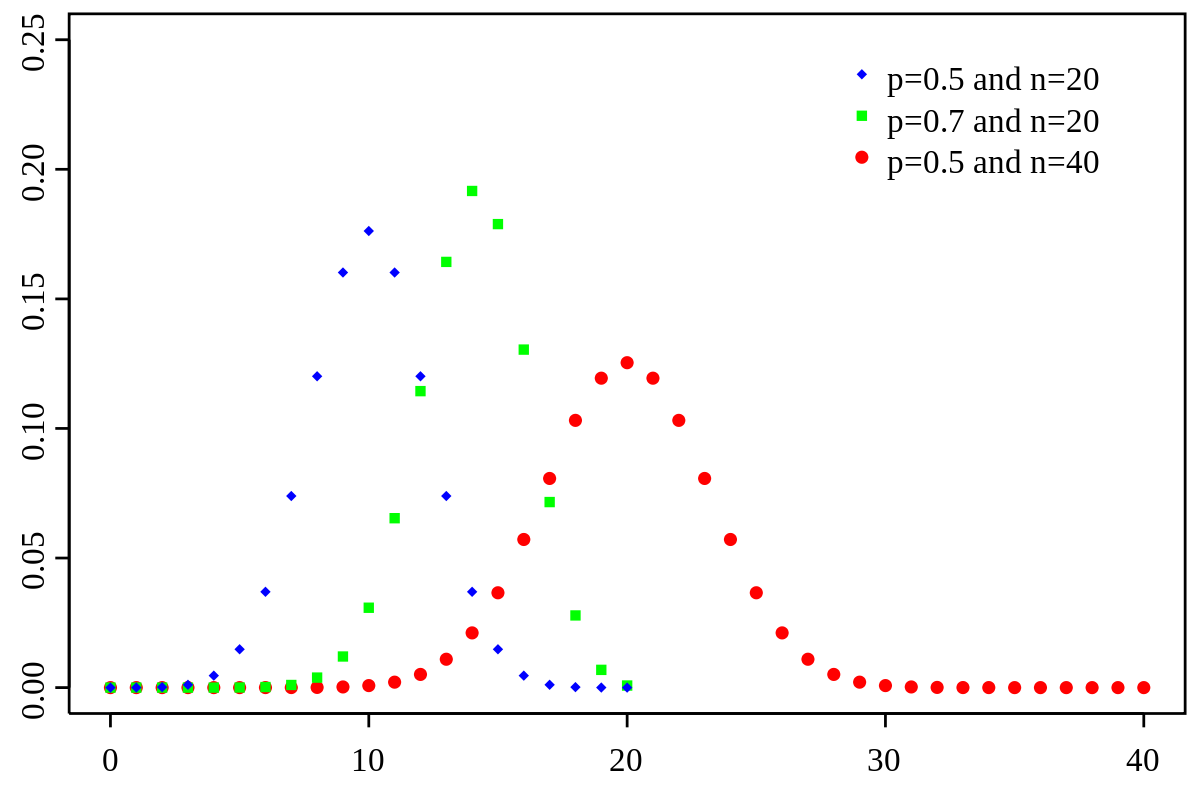
\includegraphics[width=16cm]{Images/Binomial distribution.png}
    \caption{Examples of Binomial Distributions}
    \label{fig:binomial distribution}
\end{figure}

\begin{note}
\end{note}
When $n = 1$, the probability distribution of $X$ becomes $f_X(x) = p^x (1-p)^{1-x},\ x = 0,1$, which is identical to Bernoulli Distribution. Hence, we can say that Bernoulli Distribution is a special case of the binomial distribution. \\
A random variable $X$ is a $B(n,p)$ random variable \textbf{if, and only if,} $X = X_1 + X_2 + \dots + X_n$ where $X_1, \dots , X_n$ are independent random variables, each of which follows the same Bernoulli distribution with the success probability $p$. By convention, we say "$X_1, \dots, X_n$ are independent and identically distributed (i.i.d.) $Bernoulli(p)$ random variables". \\
This is particularly useful to derive the expectation and variance of $X$, as given below.


\thm{Mean and Variance of Binomial Distributions
If $X$ has a binomial distribution with parameters $n$ and $p$ (i.e., $X \sim B(n,p)$), then the mean and variance of $X$ are
\begin{equation*}
\begin{split}
    \mu &= E(X) = np \\
    \sigma^2 &= V(X) = np(1 - p) = npq
\end{split}
\end{equation*}
}
The above formula can be derived by calculating the expected value and variance for each of the individual Bernoulli trial and then adding all of them up. It is always true that if $X = X_1 + X_2 + \dots + X_n$, then $E[X] = E[X_1] + E[X_2] + \dots + E[X_n]$. Moreover since we know that all of $X_1$ through $X_n$ are independent, the covariance of any two of them is zero and so, $V(X) = V(X_1) + V(X_2) + \dots + V(X_n)$. We already know that the expectation for any one trial is $p$ and the variance of any one trial is $pq$ (using Bernoulli trial), hence we easily observe that for $n$ trials, the expectation is $np$ and the variance is $npq$.
\begin{note}[Conditions for a Binomial Experiment]
\end{note}
\begin{enumerate}
    \item It consists of $n$ repeated Bernoulli trials
    \item Only 2 possible outcomes: success and failure in each trial
    \item $P(success) = p$ is the same constant in each trial, i.e., the number of trials previously performed or the outcomes of earlier trials should not affect the probability of success of any trial (e.g. Any experiment "without replacement" is likely to be not a Bernoulli distribution since the successive trials need not be independent). 
    \item Trials are independent
    \item The random variable $X$ is the number of successes among the $n$ trials in a binomial experiment
\end{enumerate}
Only if all the above conditions are met, $X \sim B(n,p)$.

\begin{note}[Derivation of pmf of Binomial distribution]
\end{note}
Consider a specific realization of $X_1, X_2, \dots, X_n$ namely $x_1, x_2, \dots, x_n$ such that $\sum_{i = 1}^n x_i = x$. Note the independence of $X_1, X_2, \dots, X_n$ and that they are all $Bernoulli(p)$ random variables. So, we have,
\begin{equation*}
\begin{split}
    P(X_1 = x_1, X_2 = x_2, \dots, X_n = x_n) &= P(X_1 = x_1)P(X_2 = x_2)\dots P(X_n = x_n) \\
    &= \prod_{i = 1}^{n} p^{x_i}q^{1-x_i} = p^{\sum_{i = 1}^n x_i} q^{n -\sum_{i = 1}^n x_i } \\
    &= p^x q^{n - x}
\end{split}
\end{equation*}
$\sum_{i = 1}^n x_i = x$ on the one hand means that the realized value for the corresponding $X$ is $x$; on the other hand, it means that out of $n$ trials, we get $x$ successes. There are $\binom{n}{x}$ number of such sequences, as we can think of it as choosing $x$ positions to take value 1 out of a length $n$ sequence, and other positions will be 0. As a consequence by nothing that for different choices of $x_1, x_2, \dots , x_n$, $\{X_1 = x_1, X_2 = x_2, \dots , X_n = x_n\}$ are sets of mutually exclusive events, we have
\begin{equation*}
    \begin{split}
        P(X = x) &= P\left( \bigcup_{x_1, \dots, x_n : \sum x_i = x} \{X_1 = x_1, X_2 = x_2 \dots, X_n = x_n \} \right) \\
        &= \sum_{x_1, \dots, x_n : \sum x_i = x} P(X_1 = x_1, X_2 = x_2, \dots, X_n = x_n) \\
        &= \sum_{x_1, \dots, x_n : \sum x_i = x} p^x q^{n-x} = \binom{n}{x}p^x q^{n-x}
    \end{split}
\end{equation*}
\begin{note}
\end{note}
If $X$ and $Y$ are 2 \textbf{independent} random variables that follow Binomial distributions with the same probability of success but possibly differing number of trials, $X + Y$ is also a binomial distribution with the same probability of success but the number of trials equal to the sum of the trials of the two random variables. That is, if $X \sim B(n,p), Y \sim B(m,p)$ then, $ X + Y \sim B(n + m, p)$. (Intuitively this should make sense since they are independent)
\begin{note}[Hypergeometric Distribution]
\end{note}
The hypergeometric distribution is a discrete probability distribution that describes the probability of $k$ successes (random draws for which the object drawn has a specified feature) in $n$ draws, without replacement, from a finite population of size $N$ that contains exactly $K$ objects with that feature, wherein each draw is either a success or a failure. In contrast, the binomial distribution describes the probability of $k$ successes in $n$ draws with replacement. \\
A random variable $X$ follows the hypergeometric distribution if its probability mass function (pmf) is given by:
$$
p_X(k) = P(X = k) = \dfrac{\binom{K}{k}\binom{N - K}{n - k}}{\binom{N}{n}}
$$
where,
\begin{itemize}
    \item $N$ is the population size 
    \item $K$ is the number of success states in the population
    \item $n$ is the number of draws (quantity each trial)
    \item $k$ is the number of observed successes
\end{itemize}

\subsection{Negative Binomial Distribution}
Let us consider an experiment where the properties are the same as those listed for a binomial experiment with the exception that the trials will be repeated until a fixed number of successes occur. \\
We are interested in the probability of the $k^{th}$ success occurring on the $x^{th}$ trial where $x$ is the random variable. Notice how this is different from a binomial distribution in which case we are interested in the probability of $x$ successes in $n$ trials. \\
\begin{definition}[Negative Binomial Distribution] 
Let $X$ be a random variable representing the number of trials to produce the $k$ successes in a sequence of independent Bernoulli trials. The random variable $X$ is said to follow a Negative Binomial Distribution with parameters k and p (i.e. $NB(k,p)$). The probability function of $X$ is given by:
$$
P(X = x) = f_X(x) = 
\begin{cases}
\binom{x-1}{k-1}p^x q^{x-k}, \qquad \text{for } x = k, k + 1, k + 2, ... \\
0, \qquad \text{otherwise}
\end{cases}
$$
\end{definition}
An example of negative binomial distribution would be to find the probability that the 5th success occurs in the 7th trial. So, for this to occur, we need to find the probability of getting 4 successes in the first 6 trials and then multiply that by the probability of getting a success (for the 7th trial).
\thm{Mean and Variance of Negative Binomial Distribution \\
If $X \sim NB(k,p)$, i.e., if $X$ follows a negative binomial distribution with parameters $k$ and $p$, then,
\begin{equation*}
\begin{split}
    \mu &= E[X] = \dfrac{k}{p} \\
    \sigma^2 &= Var(X) = \dfrac{(1-p)k}{p^2}
\end{split}
\end{equation*}
}
\subsection{Geometric Distribution}
A geometric distribution is a special kind of negative binomial distribution in which we find the number of trials required to have the first success. In other words, we set the parameter $k = 1$. So, whenever we talk about a geometric distribution, there is only 1 parameter $p$, which refers to the probability of success for any individual trial. We write $X \sim Geom(0.4)$ to denote that $X$ follows a geometric distribution with probability of success = 0.4. \\
Geometric distribution represents the probability of the number of successive failures before a success is obtained in a Bernoulli trial. That is, in a geometric distribution, a Bernoulli trial is repeated until a success is obtained and then stopped. \\
The probability and cumulative probability functions for a geometric distribution are:
\begin{equation*}
    \begin{split}
        P(X = x) &= p(1-p)^{x-1} \\
        P(X \leq x) &= 1 - (1-p)^x
    \end{split}
\end{equation*}
An easy way to understand the cumulative probability function is to think of the complement event: What is the probability that all the first $x$ trials result in failure? That would be $(1-p)^x$. So, the probability that at least 1 success occurs in the first $x$ trials is just $1 - (1-p)^x$ \\
Obviously, the mean of the geometric distribution is $\dfrac{1}{p}$ and the variance is $\dfrac{1-p}{p^2}$ since $k = 1$.
\begin{note}
\end{note}
Another way to describe a negative binomial distribution is to consider it as the sum of many geometric random variables. For example, $Y \sim NB(k,p)$ and $X_i = Geom(p), i = 1,2,3,\dots, k$. Then, it is possible to write $Y = X_1 + X_2 + \dots + X_k$. So, it follows that $E[Y] = E[X_1] + E[X_2] + \dots E[X_n] = \dfrac{1}{p} + \dfrac{1}{p} + \dots + \dfrac{1}{p} = \dfrac{k}{p}$. Also, $Var(Y) = Var(X_1) + Var(X_2) + \dots + Var(X_k) = \dfrac{1-p}{p^2} + \dfrac{1-p}{p^2} + \dots + \dfrac{1-p}{p^2} = \dfrac{(1-p)k}{p^2}$ 
\section{Poisson Distribution}
\begin{definition}[Poisson Experiments]
Experiments yielding numerical values of a random variable $X$, \textbf{the number of successes occurring during a given time interval or in a specified region}, are called Poisson experiments. They must satisfy the following conditions:
\begin{enumerate}
    \item The number of successes occurring in one time interval or specified region are \textbf{independent} of those occurring in any other disjoint time interval or region of space
    \item The \textbf{probability of a single success} occurring during a very short time interval or in a small region is \textbf{directly proportional to the length of the time interval} or the size of the region and does not depend on the number of successes occurring outside this time interval or region.
    \item The \textbf{probability of more than one success} occurring in such a short time interval or falling in such a small region is \textbf{negligible}.
\end{enumerate}
The given time interval, $t$, may be of any length, such as a minute, a day, a week, or even a year
\end{definition}
Examples of Poisson experiment: generate observations for the random variable $X$ representing the number of telephone calls in an hour received by an office, or the number of postponed games due to rain during a football season. \\
The specified region could be a line segment, an area, a volume, or perhaps a piece of material. In this case, $X$ might represent the number of mushrooms in a plot of land, the number of bacteria in a given culture, or the number of typing errors in a page.

\begin{definition}[Poisson Distribution]
The number of successes $X$ in a Poisson experiment is called a Poisson random variable. The probability distribution of the Poisson random variable $X$, is called the Poisson distribution and the probability function is given by 
$$
f_X(x) = P(X = x) = 
\begin{cases}
\dfrac{e^{-\lambda}\lambda^x}{x!}, \text{ for }x = 0,1,2,3,... \\
0, \text{ otherwise}
\end{cases}
$$
where $\lambda$ is the average number of successes occurring in the given time interval or specified region and $e \approx 2.71828$ is called Euler's number.
\end{definition}
\begin{figure}[ht]
    \centering
    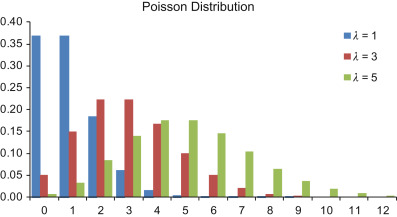
\includegraphics[width = 16cm]{Images/Poisson Distribution.jpg}
    \caption{Example of some Poisson Distributions}
    \label{fig:my_label}
\end{figure}
We write $X \sim P(\lambda)$ to indicate that $X$ follows a Poisson Distribution with parameter $\lambda$.
\thm{Mean and Variance of Poisson Random Variable \\
IF $X$ has a Poisson distribution with parameter $\lambda$, then
\begin{equation*}
    \begin{split}
        \mu &= E[X] = \lambda \\
        \sigma^2 &= V(X) = \lambda
        \end{split}
\end{equation*}}
\begin{note}[Density Manipulation]
\end{note}
The method for deriving these results is called density manipulation. The fundamental idea is simple: for any arbitrary probability function $f(x)$,
\begin{itemize}
    \item if the distribution is discrete, $\sum_{x \in \{x|f(x)>0\}} f(x) = 1$
    \item if the distribution is continuous $\int_{\infty}^{\infty} f(x) = 1$
\end{itemize}
Both of the above follow directly from the axioms of probability (since the total probability must be 1). \\
Proof of mean and variance of Poisson Random Variable:
\begin{equation*}
    \begin{split}
        E(X) &= \sum_{x = 0}^{\infty} x \dfrac{e^{-\lambda}\lambda^x}{x!} \\
        &= \sum_{x = 1}^{\infty} \dfrac{e^{-\lambda}\lambda^x}{(x-1)!} \\
        &= \lambda \sum_{y = 0}^{\infty} \dfrac{e^{-\lambda}\lambda^y}{y!} \qquad \text{where } y = x - 1 \\
        &= \lambda \qquad \text{because } \sum_{y = 0}^{\infty}\dfrac{e^{-\lambda}\lambda^y}{y!} = \sum_{y = 0}^{\infty} f_Y(y) = 1, \text{where } Y \sim P(\lambda) 
    \end{split}
\end{equation*}
In other words, $\sum_{y = 0}^{\infty}\dfrac{e^{-\lambda}\lambda^y}{y!} = 1$ because it is a probability function and its sum over all possible values must be 1. \\
The proof of variance of Poisson Distribution is obtained by first finding $E[X(X - 1)]$.
\begin{equation*}
    \begin{split}
        E[X(X - 1)] &= \sum_{x = 0}^{\infty}x(x-1)\dfrac{e^{-\lambda}\lambda^x}{x!} \\
        &= \sum_{x = 2}^{\infty}\dfrac{e^{-\lambda}\lambda^x}{(x-2)!} \\
        &= \lambda^2 \sum_{y = 0}^{\infty}\dfrac{e^{-\lambda}\lambda^y}{y!} \qquad \text{where } y = x - 2 \\
        &= \lambda^2 \\
        \text{Now, } \\
        V(X) &= E[X^2] - [E(X)]^2 \\
        &= E[X(X - 1)] + E[X] - [E(X)]^2 \qquad \text{due to linearity of expectation}\\
        &= \lambda^2 + \lambda - \lambda^2 \\
        &= \lambda
    \end{split}
\end{equation*}
\begin{note}[Properties of the Poisson Distribution]
\end{note}
\begin{itemize}
    \item Let $X$ follows $Poisson(\lambda_1)$ distribution. Let $Y$ follows $Poisson(\lambda_2)$ distribution. If $X$ and $Y$ are independent, then $X + Y \sim Poisson(\lambda_1 + \lambda_2)$. \\
    For example, if the average number of robberies in a day is 4, then the average number of robberies in 2 days will be 8, assuming that robberies occurring on different days are independent.
    \item Let $X$ be the number of occurrences of an event in a period of time $T$; it has the $Poisson(\lambda)$ distribution. If $Y$ is the number of occurrences of the event in a period of time $tT$, then $Y \sim Poisson(t\lambda)$.
\end{itemize}
\begin{note}[Comparison between Distributions]
\end{note}
Binomial Distribution, Negative Binomial distribution, and the Poisson distribution are all founded on Bernoulli trials. Their corresponding random variables $X$, however are defined differently:
\begin{itemize}
    \item For Binomial distribution, $X$ is defined to be the number of successes out of $n$ independent Bernoulli trials with $p$ constant for all trials.
    \item For Negative Binomial distribution, $X$ is defined to be the number of trials needed so that we achieve $k$ successes.
    \item For Poisson distribution, $X$ is defined to be the number of successes in a period of time or in a specific region.
\end{itemize}

\section{Poisson Approximation to the Binomial Distribution}
\thm{Let $X$ be a \textbf{Binomial} random variable with parameters $n$ and $p$. That is,
$$
P(X = x) = f_X(x) = \binom{n}{x}p^x q^{n-x}, \text{ where } q = 1 - p
$$
Suppose that $n \rightarrow \infty$ and $p \rightarrow 0$ in such a way that $\lambda = np$ remains a constant as $n \rightarrow \infty$. Then, $X$ will have approximately a Poisson distribution with parameter $np$. That is,
$$
\lim_{p \rightarrow 0, \ n \rightarrow \infty}\  P(X = x) = \dfrac{e^{-np}(np)^x}{x!}
$$}
\begin{note}
\end{note}
If $p$ is close to 1, we can still use Poisson distribution to approximate binomial probabilities by interchanging what we have defined to be a success and a failure so that $p$ becomes a value close to zero.
\begin{note}
\end{note}
The reason we can approximate a Binomial distribution using a Poisson distribution because for small values of $p$, the binomial distribution is right skewed (with the right-tail being longer). This makes intuitive sense because the lower the probability of success, the smaller the expected number of successes. Moreover, even the Poisson distribution is right-skewed. On the other hand, when the probability of success is close to $\dfrac{1}{2}$, the binomial distribution becomes nearly symmetric, and hence the normal distribution can better approximate it.

\section{Continuous Uniform Distribution}
\begin{definition}[Continuous Uniform Distribution]
A continuous random variable is said to have a uniform distribution over the interval $[a,b]$, $-\infty < a < b < \infty$, denoted by $U(a,b)$, if its probability density function is given by,
$$
f_X(x) = \begin{cases}
\dfrac{1}{b-a}, \text{ for } a \leq x \leq b \\
0, \text{ otherwise}
\end{cases}
$$
This distribution is also referred to as rectangular distribution because of the rectangular shape of the p.d.f.
\end{definition}
\begin{figure}[ht]
    \centering
    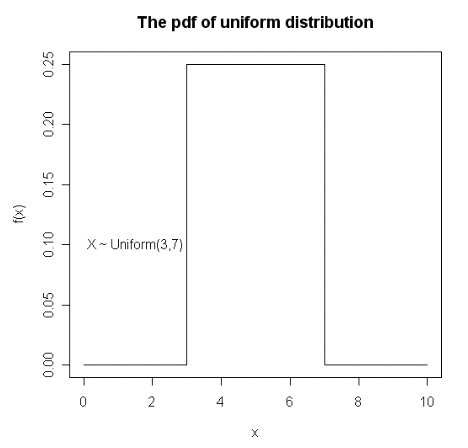
\includegraphics[width = 10cm]{Images/continuous uniform distribution.png}
\end{figure}

\thm{Mean and Variance of Continuous Uniform Distribution \\ 
If $X$ is uniformly distributed over $[a,b]$, then
\begin{equation*}
    \begin{split}
        E[X] &= \dfrac{a + b}{2} \\
        V(X) &= \dfrac{(b-a)^2}{12}
    \end{split}
\end{equation*}
}
Proof:
\begin{equation*}
    \begin{split}
        E[X] &= \int_{a}^{b} x \dfrac{1}{b-a}dx = \dfrac{1}{b-a} \left[ \dfrac{x^2}{2}\right]_{x = a}^{x = b} \\
        &= \dfrac{1}{b-a}\dfrac{b^2 - a^2}{2} \\
        &= \dfrac{a + b}{2} \\
        \text{Also, } \\
        E[X^2] &= \int_{a}^{b} x^2 \dfrac{1}{b-a}dx = = \dfrac{1}{b-a} \left[ \dfrac{x^3}{3}\right]_{x = a}^{x = b} \\
        &= \dfrac{1}{b-a}\dfrac{b^3 - a^3}{3} \\
        &= \dfrac{a^2 + ab + b^2}{3} \\
        \text{Then, } \\
        V(X) &= E[X^2] - (E[X])^2 \\
        &= \dfrac{a^2 + ab + b^2}{3} - \dfrac{(a + b)^2}{4} \\
        &= \dfrac{(b-a)^2}{12}
    \end{split}
\end{equation*}
Keep in mind that these formulae are applicable only when the distribution is defined on a single interval.
\begin{note}[c.d.f. of a uniformly distributed random variable]
\end{note}
Let $X$ be a uniformly distributed random variable between $[a,b]$. Then,
\begin{equation*}
    \begin{split}
        F_X(x) &= \int_{-\infty}^{x} f_X(t)dt \\
        &= \begin{cases}
        \int_{-\infty}^{x} 0 dt, \text{ for } x < a \\
        \int_{-\infty}^{a} 0 dt +  \int_{a}^{x} \dfrac{1}{b-a} dt, \text{ for } a \leq x \leq b \\
        \int_{-\infty}^{a} 0 dt + \int_{a}^{b} \dfrac{1}{b-a} dt + \int_{b}^{x} 0 dt, \text{ for } b < x
        \end{cases} \\
        &= 
        \begin{cases}
        0, \text{ for } x < a \\
        \dfrac{x-a}{b-a} \text{ for } a \leq x \leq b \\
        1, \text{ for } b < x
        \end{cases}
    \end{split}
\end{equation*}

\section{Exponential Distribution}
\begin{definition}[Exponential Distribution]
\end{definition}
A continuous random variable $X$ assuming all non-negative values is said to have an exponential distribution with parameter $\alpha > 0$ if its probability density function is given by
$$
f_X(x) = \begin{cases}
\alpha e^{-\alpha x}, \text{ for } x > 0 \\
0, \text{ otherwise}
\end{cases}
$$
Note that $\int_{-\infty}^{\infty} f_X(x)dx = 1$.

\thm{Mean and Variance of Exponential RV \\ 
If $X$ has an exponential distribution with parameter $\alpha > 0$, then
\begin{equation*}
    \begin{split}
        E[X] &= \dfrac{1}{\alpha} \\
        V(X) &= \dfrac{1}{\alpha^2}
    \end{split}
\end{equation*}}
The proof is very similar to that of continuous uniform distribution and is left an exercise to the reader.

\begin{note}
\end{note}
The p.d.f. can be written in the form $f_X(x) = \dfrac{1}{\mu} e^{\frac{-x}{\mu}}$, for $x > 0$ and 0 otherwise. Then, $E[X] = \mu$ and $V(X) = \mu^2$.

\thm{No Memory Property of Exponential Distribution \\
Suppose that $X$ has an exponential distribution with parameter $\alpha > 0$. Then, for any 2 positive numbers $s,t$, we have
$$
P(X > s + t | X > s) = P(X > t)
$$}
It can be proved using the formulae for conditional probability distributions and is a good exercise for the reader to revise. \\
The above theorem states that the exponential distribution has no memory in the following sense: Let $X$ denote the life length of a bulb. Given that the bulb has lasted $s$ time units (i.e. $X > s$) then the probability that it will last for the next $t$ units (i.e. $X > s + t$) is the same as the probability that it would have lasted for the first $t$ units if it were brand new.\\
This property usually refers to the cases when the distribution of a "waiting time" until a certain event does not depend on how much time has elapsed already. To model memoryless situations accurately, we must constantly 'forget' which state the system is in: the probabilities would not be influenced by the history of the process. For example, assume the bus frequency follows an exponential distribution. If you have been waiting at a bus stop for 10 minutes, what is the probability that you have to wait for 5 more minutes? This probability will be the same for someone who just arrived at the bus stop 10 minutes after you came. So, the expected amount of waiting time does not depend on the time for which you have already been waiting for. \\ Apart from the exponential distribution, the only other distribution which has this memoryless property is the geometric distribution (which makes sense because your odds of getting a success do not increase even though you have performed many trials before it - for example, you toss a coin 3 times and you get tails all 3 times (which you consider to be a failure). Your chances of getting a head (success) remain the same the next time you throw it too).

\begin{note}[c.d.f of the exponential distribution]
\end{note}
Let $X$ be a continuous random variable following an exponential distribution with parameter $\alpha$. Then, for $x \geq 0$,
$$
F_X(x) = P(X \leq x) = \int_{0}^{x} \alpha e^{-\alpha t} dt = \left[-e^{-\alpha t}\right]_{t = 0}^{t = x} = 1 - e^{-\alpha x},
$$ and 0 otherwise. \\
Hence, $P(X > x) = e^{-\alpha x}$, for $x > 0$. \\ \hfill \\
Exponential distribution is popularly used to model the survival (recovery) time of a patient in the medical research, where $P(X > t) = 1 - F_X(t)$ is called the \textbf{survival function} It is the probability that the survival (recovery) time of a patient is greater than $t$.
\begin{note}[Application of the Exponential Distribution]
\end{note}
The exponential distribution is frequently used as a model for the distribution of times between the occurrence of successive events such as customers arriving at a service facility or calls coming into a switchboard.

\section{Normal Distribution}
\begin{definition}[Normal Distribution]
The random variable $X$ assuming all real values, $-\infty < x < \infty$ has a normal (or Gaussian) distribution if its probability density is given by
$$
f_X(x) = \dfrac{1}{\sigma \sqrt{2\pi}} exp\left( - \dfrac{(x-\mu)^2}{2\sigma^2}\right), \text{ for } -\infty < x < \infty
$$ where $-\infty < \mu < \infty $ and $\sigma > 0$.
It is denoted by $N(\mu, \sigma^2)$, and $\mu$ and $\sigma^2$ are called the parameters of the normal distribution.
\end{definition}

\subsection{Properties of the Normal Distribution}
\begin{enumerate}
    \item The graph of this distribution is of bell-shaped and called the normal curve. It is symmetrical about the vertical line $x = \mu$.
    \item The mean, median, and mode of the normal distribution are the same and equal to $\mu$.
    \item The maximum point occurs at $x = \mu$ and its value is $\dfrac{1}{\sigma \sqrt{2\pi}}$.
    \item The normal curve approaches the horizontal axis asymptotically as we proceed in either direction away from the mean.
    \item The total area under the curve and above the horizontal axis is equal to 1 (since it is a probability density function)
    \item It can be shown that $E[X] = \mu$ and $V(X) = \sigma^2$.
    \item 2 normal curves are identical in shape if they have the same $\sigma^2$. But they are centered at different positions when their means are different.
    \item As $\sigma$ increases, the curve flattens, and as $\sigma$ decreases, the curve steepens/sharpens.
    \item If $X \sim N(\mu, \sigma^2)$, and if $Z = \dfrac{X - \mu}{\sigma}$, then $Z \sim N(0,1)$. That is, $Z$ follows the $N(0,1)$ distribution. Then, $E[Z] = 0$ and $V(Z) = 1$. We say that $Z$ has a standardized normal distribution. That is, the p.d.f. of $Z$ may be written as: $f_Z(z) = \dfrac{1}{\sqrt{2\pi}} exp\left( - \dfrac{z^2}{2}\right)$. \\
    The importance of the standardized normal distribution is the fact that it is tabulated. Whenever $X$ has distribution $N(\mu,\sigma^2)$, we can always simplify the process of evaluating the values of $P(x_1 < X < x_2)$ by using the transformation $Z = \dfrac{X - \mu}{\sigma}$. Then,
    $x_1 < X < x_2$ is equivalent to $\dfrac{x_1 - \mu }{\sigma} < Z < \dfrac{x_2 - \mu }{\sigma}$. \\
    Let $z_1 = \dfrac{x_1 - \mu }{\sigma}$ and $z_2 = \dfrac{x_2 - \mu }{\sigma}$. Then, $P(x_1 < X < x_2) = P(z_1 < Z < z_2)$
    \item The density is symmetric about $\mu$, which is the expectation and median of the distribution. One direct consequence is that $P(X \leq \mu) = P(X \geq \mu) = 0.5$. $\mu$ is also called the location parameter, which determines the location of the center of the distribution.
    \item $\sigma^2 = V(X)$ is the shape parameter (also called the dispersion parameter in literature), which determines the shape of the density function.
    \item For any value of $\mu, \sigma^2$, the density if positive for all $x \in \mathbb{R}$. It get closer and closer to (but never equal to) 0, when x approaches $\infty$ or $-\infty$.
    \item The standardization $Z = \dfrac{X - \mu}{\sigma}$ is very important. The density becomes symmetric about 0. That is, for any $z \in \mathbb{R}, \ P(Z \leq -z) = P(Z \geq z)$. $E[Z] = 0$ and $V(Z) = 1$. With this standardization, for $x_1 < x_2$, $P(x_1 < X < x_2)$ (with $\mu$ and $\sigma^2$ being any given values) can always be obtained from the table for $Z$.
    \item For any normal random variable $X$, the probability that $X$ is within $c$ standard deviations from the mean value is always deterministic, where $c > 0$ is a known constant. In particular, if $X \sim N(\mu, \sigma^2)$, 
    $$
    P(\mu - c\sigma < X < \mu + c\sigma) = P(-c < \dfrac{X - \mu}{\sigma} < c) = P(|Z| < c),
    $$ which does not depend on $\mu$ and $\sigma$. Observe that $\dfrac{X - \mu}{\sigma}$ gives you exactly the number of standard deviations that the random variable is away from its expected value.\\
    For example, the probability that a normal random variable is within 1 standard deviation of its mean is 68.27\%, within 2 standard deviations is 95.45\%, and within 3 standard deviations is 99.73\%. So, if the IQ scores of a population follow a normal distribution with mean = 100 and standard deviation = 15, then we can say that 68.27\% of the population has an IQ score between 85 and 115, and 99.73\% of the population has an IQ score between 55 and 145.
    \item For 2 \textbf{independent normal random variables} $X \sim N(\mu_1, \sigma_{1}^2)$ and $Y \sim N(\mu_2, \sigma_{2}^2)$, then $X + Y \sim N(\mu_1 + \mu_2, \sigma_{1}^2 + \sigma_{2}^2)$. Also, $X - Y \sim N(\mu_1 - \mu_2, \sigma_{1}^2 + \sigma_{2}^2)$
\end{enumerate}
\begin{note}
\end{note}
It is important to remember that the last point is not true for any kind of general distribution. For example, if $X \sim exp(\lambda)$ and $Y \sim exp(\lambda)$ and $X$ and $Y$ are independent, $X + Y$ does not follow an exponential distribution.
\begin{figure}[ht]
    \centering
    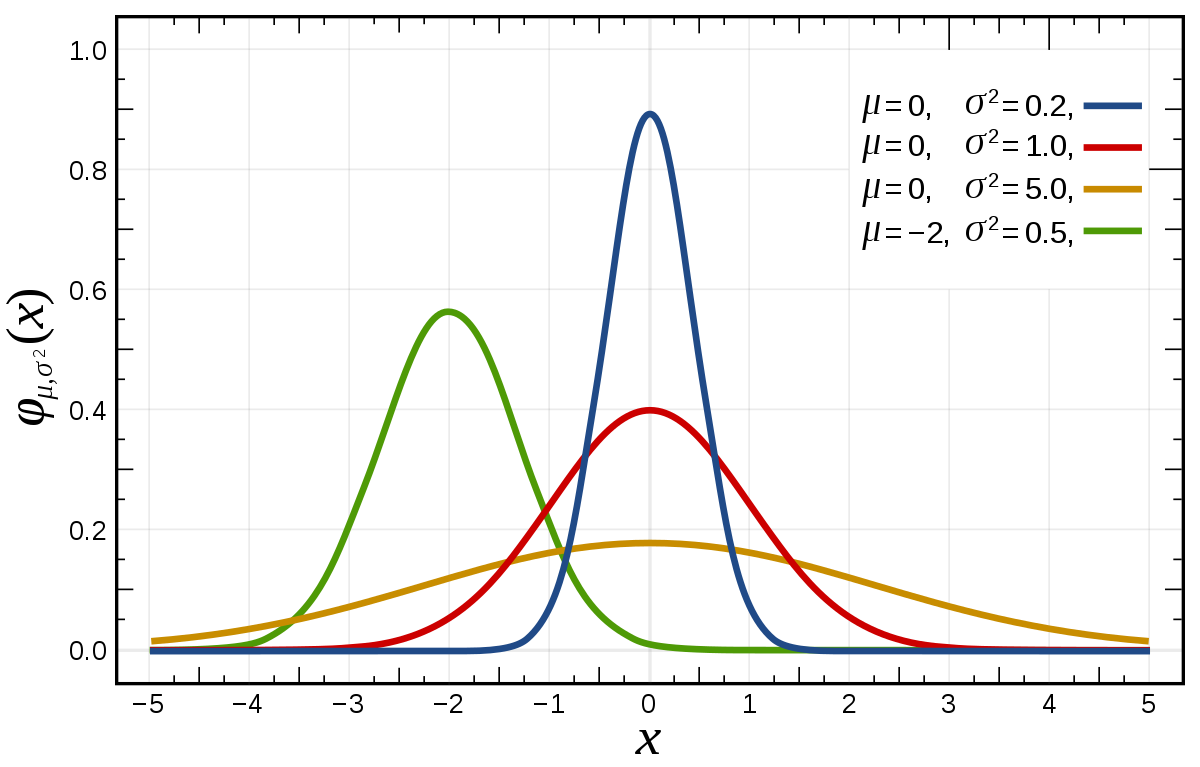
\includegraphics[width = 12cm]{Images/normal.png}
    \caption{Examples of Normal Distribution}
    \label{fig:my_label}
\end{figure}
\subsection{Application of Standardisation}
It is very important to standardise the values before comparing two distributions that follow a normal distribution. The value of $Z$ tells us how far the data point is from the mean (in terms of the number of standard deviations). \\
For example, consider 2 classes - A and B - which had an examination. The distribution of marks in A followed a normal distribution with mean = 50 and standard deviation = 5. Similarly, in class B, the mean was 65 and the standard deviation was 8. Then if student p (from class A) got 60 marks and student q (from class B) got 65 marks, can we say that q is better than p? \\
No! We cannot compare how well p and q did directly without standardising their scores. It may be the case that class B had an easier paper in general or the teacher was lenient. We want to know how well p and q did compared to their class, and use that to determine who did better. So, we find the $Z$ values for both of them, 
$$
Z_p = \dfrac{60 - 50}{5} = 2, \ Z_q = \dfrac{65 - 65}{8} = 0
$$
This can be interpreted as follows: p is 2 standard deviations above the class average (which means he did better than 95\% of his class) while q is average in his class. Hence, we can conclude that p did better than q (assuming that students in both classes are randomly assigned).
\subsection{Statistical Tables}

Statistical tables give the values $\Phi(z)$ for a given $z$, where $\Phi(z)$ is the {\imp {cumulative distribution function of a standardized Normal random variable}} $Z$. It follows that $1 - \Phi(z)$ is the upper cumulative probability for a given $z$. Thus, $\Phi(z) = P(Z \leq z)$ and $1 - \Phi(z) = P(Z > z)$. \\
Some statistical tables give the $100\alpha$ percentage points, $z_\alpha$, of a standardized Normal distribution, where 
$$
\alpha = P(Z \geq z_\alpha) = \int_{z_\alpha}^{\infty}\dfrac{1}{\sqrt{2\pi}} exp \left( - \dfrac{z^2}{2}\right) dz
$$
Since the p.d.f. of $Z$ is symmetrical about 0, $P(Z \geq z_{\alpha}) = P(Z \leq -z_{\alpha}) = \alpha$
\section{Normal Approximation to the Binomial Distribution}
\begin{figure}[ht]
    \centering
    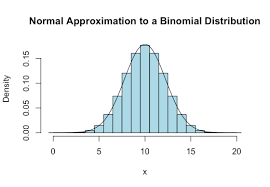
\includegraphics{Images/normal to binomial.png}
\end{figure}
When $n \rightarrow \infty$ and $p \rightarrow 0$, we may use Poisson distribution to approximate a Binomial Distribution. \\
Similarly, when $n \rightarrow \infty$ and $p \rightarrow \dfrac{1}{2}$, we can use normal distribution to approximate the binomial distribution. In fact, even when $n$ is small and $p$ is not extremely close to 0 or 1, the approximation is fairly good. We need $p$ to be close to $\dfrac{1}{2}$ because then the binomial distribution will be close to symmetric and hence, we can approximate it using normal distribution (which is always symmetric). If $p$ is close to 0 or 1, then the binomial distribution is skewed and we cannot use normal distribution to approximate it. Thus, we use Poisson (not symmetric) approximation in such cases. \\
A good rule of thumb is to use the normal approximation only when $np > 5$ and $n(1-p) > 5$.

Notice that we use the Poisson approximation and normal approximation in completely different cases, depending on the value of $p$. If $p$ is close to  0 (or 1), then we use the Poisson approximation. On the other hand, if $p$ is close to $\dfrac{1}{2}$, we use the normal approximation. It is important to keep in mind that these are just approximations and they couldn't give you the exact value. Roughly speaking, how good the approximation is depends on how the corresponding conditions are satisfied.
\thm{If X is a binomial random variable with mean $\mu = np$ and variance $\sigma^2 = np(1-p)$, then as $n \rightarrow \infty$,
$$
Z = \dfrac{X - np}{\sqrt{np(1-p)}} \text{ is approximately } \sim N(0,1)
$$. This is equivalent to saying that $X$ approximately follows $N(np, np(1-p))$ (in the above equation, we have standardized $X$ directly). }
An easy way to remember is that $X$ follows $N(\mu, \sigma^2)$ where $\mu = np$ and $\sigma^2 = np(1-p)$ in the case of binomial distribution. The 2 parameters of the normal distribution always refer to the mean and the variance respectively.
\subsection{Continuity Correction}
\begin{figure}[h]
    \centering
    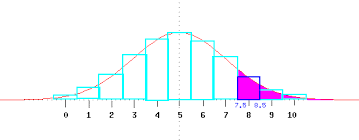
\includegraphics{Images/cont correction.png}
    \caption{Continuity Corrections}
    \label{fig:my_label}
\end{figure}

When we use normal approximation for a binomial distribution to calculate probabilities, we run into some problems. For example, how would we calculate $P(X = k)$ for some value $k$? We know that for a continuous random variable, the probability that $X$ takes on a fixed value is 0. But this is not true for a binomial distribution. Hence, we need to approximate $P(X = k)$ as being equal to $P(k - \dfrac{1}{2} < X < k + \dfrac{1}{2})$. It might be helpful to draw the bars of binomial distribution and the corresponding normal distribution to understand. \\ 
A continuity correction is the name given to adding or subtracting 0.5 to a discrete x-value.
For example, suppose we would like to find the probability that a coin lands on heads less than or equal to 45 times during 100 flips. That is, we want to find $P(X \leq 45)$. To use the normal distribution to approximate the binomial distribution, we would instead find $P(X \leq 45.5)$ because 45 is the midpoint of the bar which ranges from 44.5 to 45.5, and since we want to include the entire bar (since we are including 45), we need to consider the upper bound.
You don't need to memorize this continuity corrections if you understand when to include the point or not and use that to determine whether to add 0.5 or subtract 0.5.
We can use the following approximations in general (only when using normal distribution to approximate binomial distribution):
\begin{enumerate}
    \item $P(X = k) \approx P(k - \frac{1}{2} < X < k + \frac{1}{2})$
    \item $P(a \leq X \leq b) \approx P(a - \frac{1}{2} < X < b + \frac{1}{2})$ \\
    $P(a < X \leq b) \approx P(a + \frac{1}{2} < X < b + \frac{1}{2})$ \\
    $P(a \leq X < b) \approx P(a - \frac{1}{2} < X < b - \frac{1}{2})$ \\
    $P(a < X < b) \approx P(a + \frac{1}{2} < X < b - \frac{1}{2})$
    \item $P(X \leq c) = P(0 \leq X \leq c) \approx P(\frac{-1}{2} < X < c + \frac{1}{2})$ (because the minimum value of  $X$ in a binomial distribution is 0)
    \item $P(X > c) = P(c < X \leq n) \approx P(c + \frac{1}{2} < X < n + \frac{1}{2})$\ (because the maximum value of $X$ in a binomial distribution is $n$)
\end{enumerate}
%\section{Appendix: Statistical Table}
%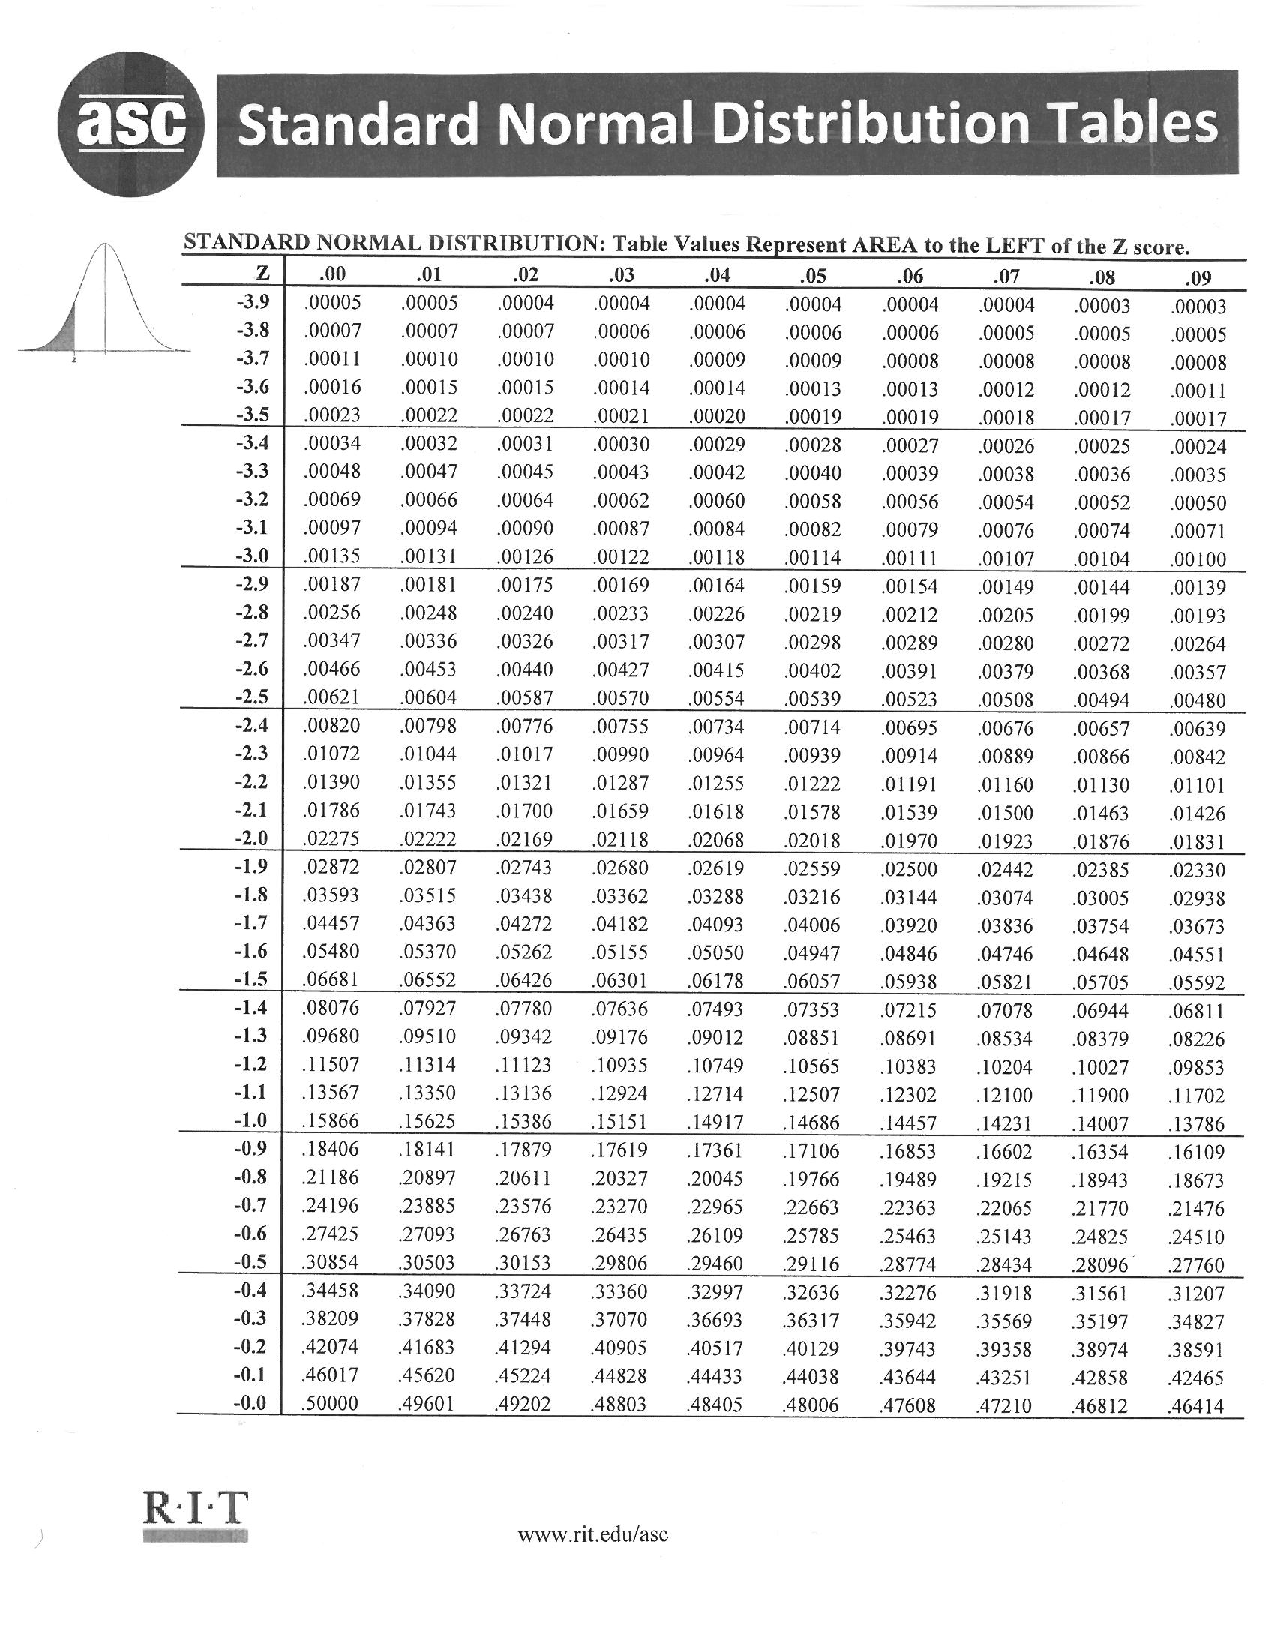
\includepdf[pages=-]{Standard Normal Distribution Table.pdf}